\documentclass[UTF8,a4paper,11pt,fontset=none]{ctexart}
\usepackage[margin=2.1cm]{geometry}
\usepackage{fontspec,booktabs,tabularx,longtable,amsmath,amssymb}
\usepackage{graphicx,float,fancyhdr,xurl,fvextra,caption,placeins}
\usepackage[hidelinks]{hyperref}
\setmainfont{DejaVu Serif}
\setsansfont{DejaVu Sans}
\setmonofont{DejaVu Sans Mono}[Scale=0.86]
\IfFontExistsTF{Noto Serif CJK SC}{\setCJKmainfont{Noto Serif CJK SC}}{\setCJKmainfont{SimSun}[AutoFakeBold=2.5]}
\IfFontExistsTF{Noto Sans CJK SC}{\setCJKsansfont{Noto Sans CJK SC}}{\setCJKsansfont{Microsoft YaHei}}
\setCJKmonofont{Microsoft YaHei}
\ctexset{section={format=\Large\bfseries},subsection={format=\large\bfseries}}
\setcounter{tocdepth}{2}
\setlength{\parskip}{0.15em}
\linespread{1.02}
\setlength{\emergencystretch}{2em}
\renewcommand{\arraystretch}{1.22}
\raggedbottom
\pagestyle{fancy}
\fancyhf{}
\fancyhead[L]{\small 互联网数据库开发 · 个人作业 2}
\fancyhead[R]{\small 2413581 黄奕浩}
\fancyfoot[C]{\thepage}
\setlength{\headheight}{14pt}
\captionsetup{font=small,labelsep=quad}
\fvset{fontsize=\footnotesize,numbers=left,numbersep=7pt,frame=none,breaklines=true,breakanywhere=true,breakautoindent=true,tabsize=2}
\newcommand{\code}[1]{\texttt{#1}}
\hypersetup{pdftitle={校园学习团队网页原型与模板选型},pdfauthor={黄奕浩 2413581}}
\begin{document}
\begin{titlepage}
\thispagestyle{empty}\centering
\vspace*{.6cm}

\includegraphics[width=.43\textwidth]{figures/nankai_logo_color.png}
\vspace{.9cm}
\rule{.88\textwidth}{.8pt}\par\vspace{.55cm}
{\fontsize{28pt}{35pt}\selectfont\bfseries 互联网数据库开发课程实验报告\par}
\vspace{.65cm}
{\fontsize{21pt}{29pt}\selectfont\bfseries 个人作业 2\quad Web前端设计\par}
\vspace{.55cm}\rule{.88\textwidth}{.8pt}\par
\vspace{1.55cm}
{\fontsize{19pt}{28pt}\selectfont\bfseries 姓名：黄奕浩\qquad 学号：2413581\par}
\end{titlepage}
{\small\tableofcontents}
\clearpage

\section{需求与信息结构}
网站面向浏览学习资源的同学和维护内容的团队成员。前台以团队展示和资源浏览为主，安排团队介绍、学习资源与留言交流；后台围绕资源管理组织表单和列表，使维护者能够查看、新增和删除资源。

访客进入首页后，先通过首屏了解团队定位，再向下浏览资源，利用关键词或分类缩小查找范围。成员介绍与留言放在资源区域之后，使内容浏览和团队交流形成连续的阅读路径。维护者进入后台后，则直接面对资源表单与现有记录，减少查找管理入口的步骤。

前后台使用一致的团队名称和栏目用语。前台强调内容介绍和阅读，后台强调数据项、状态和操作。页面通过“后台原型”和“返回前台”入口互相连接，便于查看两类用户对应的界面。

\section{页面原型设计}
\subsection{前台页面布局}
前台从上到下依次排列品牌导航、首屏介绍、学习资源、团队介绍和留言区域。导航将资源、团队和留言作为主要入口，首屏用标题、说明与按钮突出校园学习主题。资源区域位于页面中部，既能承接首屏的浏览操作，也能在进入页面后较快找到主要内容。

学习资源采用卡片形式呈现。每张卡片包含分类、标题和简短说明，三类示例内容分别对应数据库、前端和协作工具。搜索框与分类下拉框排列在卡片上方，使筛选条件与筛选结果保持在同一视觉区域。页面显示当前结果说明，帮助访客理解操作后的变化。

\begin{figure}[H]\centering
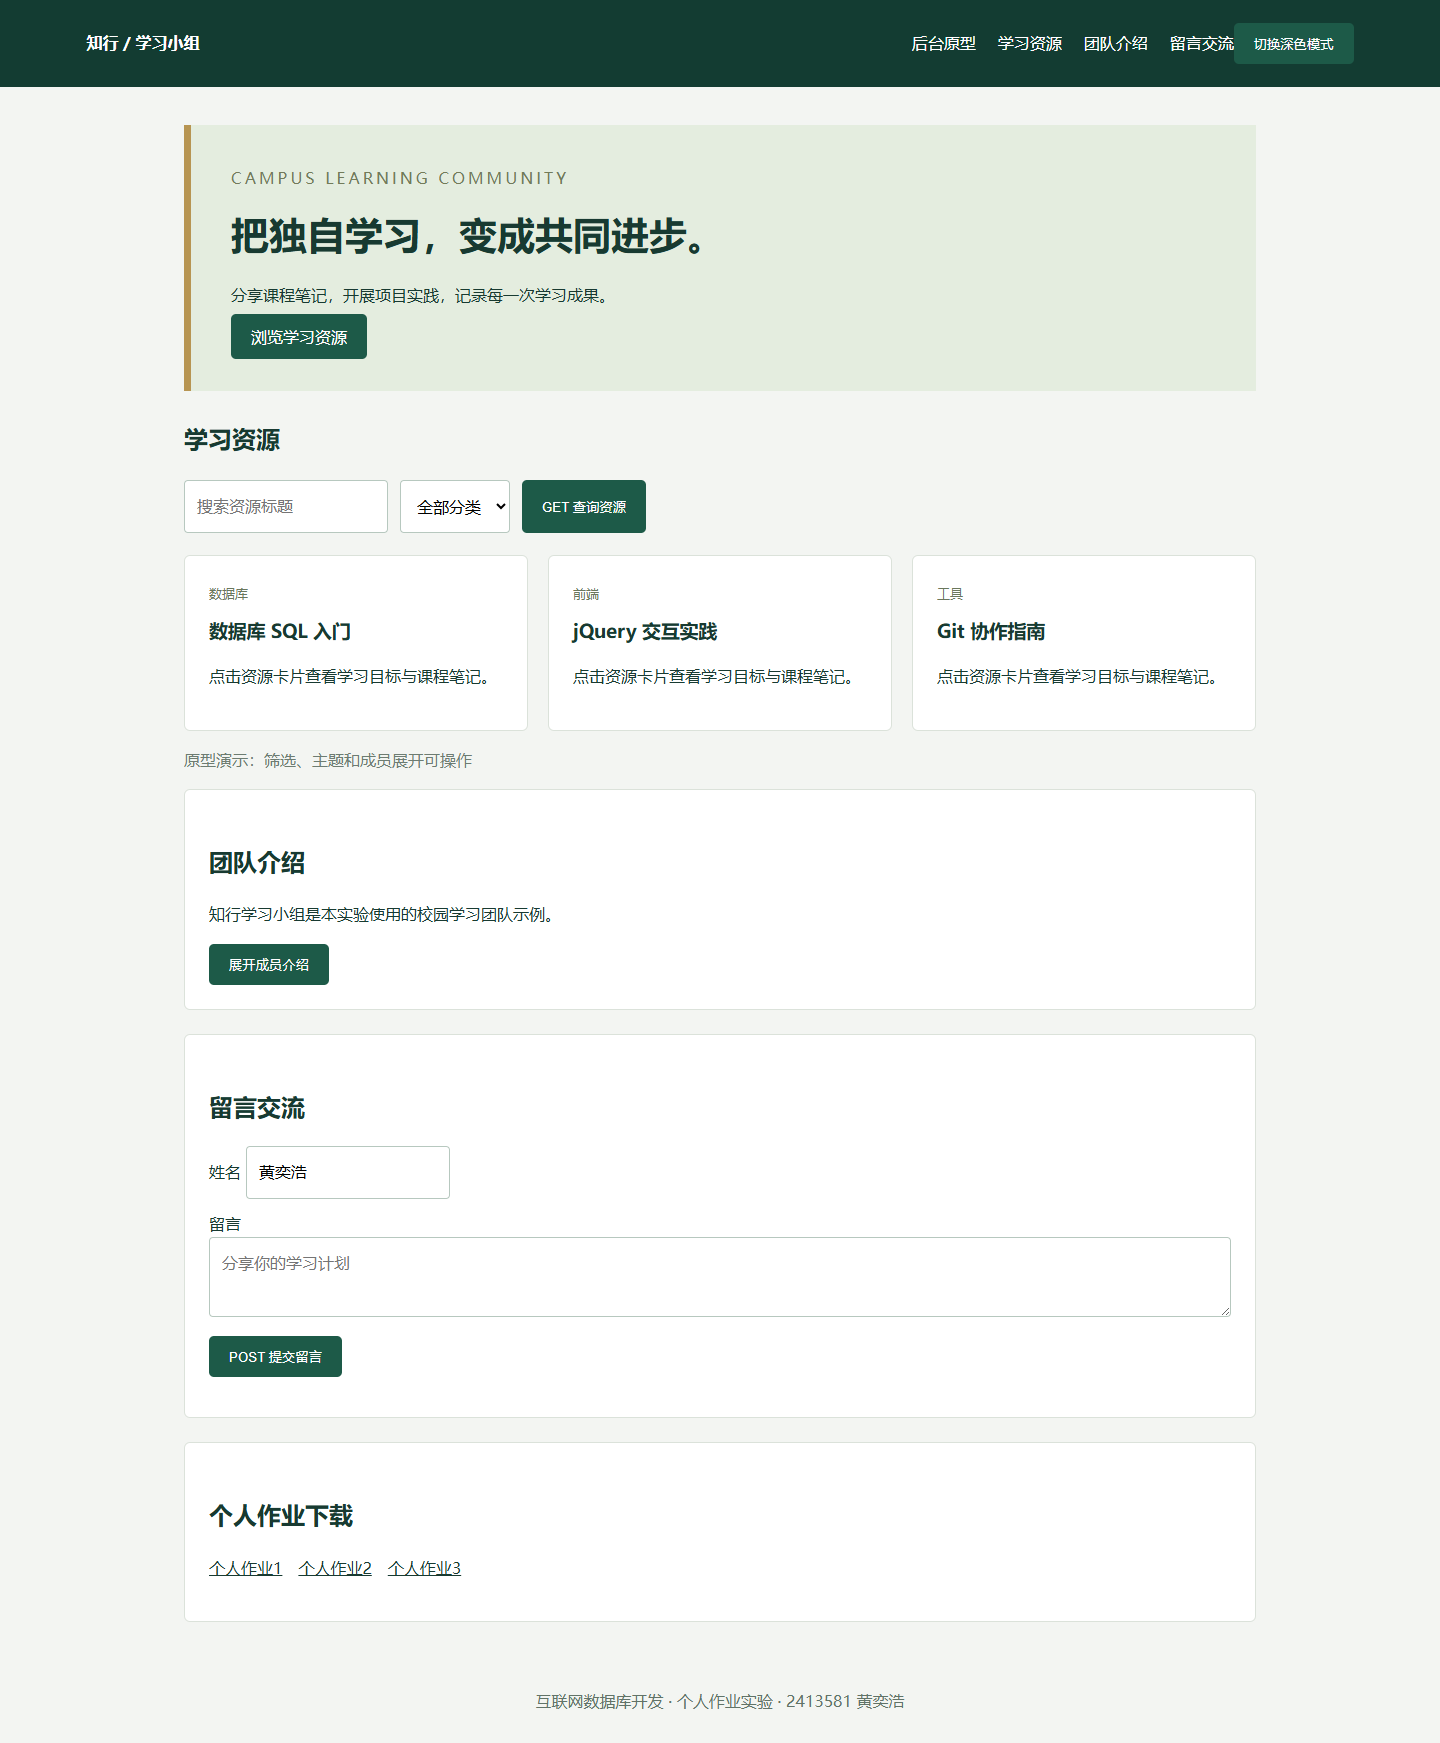
\includegraphics[width=\linewidth,height=.48\textheight,keepaspectratio]{figures/figure-01.png}
\caption{前台页面的导航、资源、团队与留言布局}
\end{figure}


页面中的搜索和分类条件共同决定显示内容。输入关键词后匹配资源标题，选择分类后进一步限制结果；清空关键词或切换回全部分类可恢复对应内容。成员介绍采用展开与收起方式显示，首屏和内容区域可切换深浅主题。留言表单包含姓名、内容和提交按钮，提交后在表单下方显示反馈，操作结果靠近触发位置。

\subsection{后台资源管理布局}
后台采用左侧导航与右侧工作区的结构。左侧集中展示资源管理、团队信息和留言审核等栏目，右侧首先放置新增资源表单，下方紧接资源列表。当前原型围绕资源管理展开，新增和删除操作均在这一工作区完成。

新增表单包含资源标题、分类和提交按钮。标题使用必填输入框，分类使用下拉选择，减少同一类别出现多种写法的情况。资源列表按标题、分类、状态和操作排列，新增后的记录沿用相同列顺序，便于对照刚才填写的内容。

\begin{figure}[H]\centering
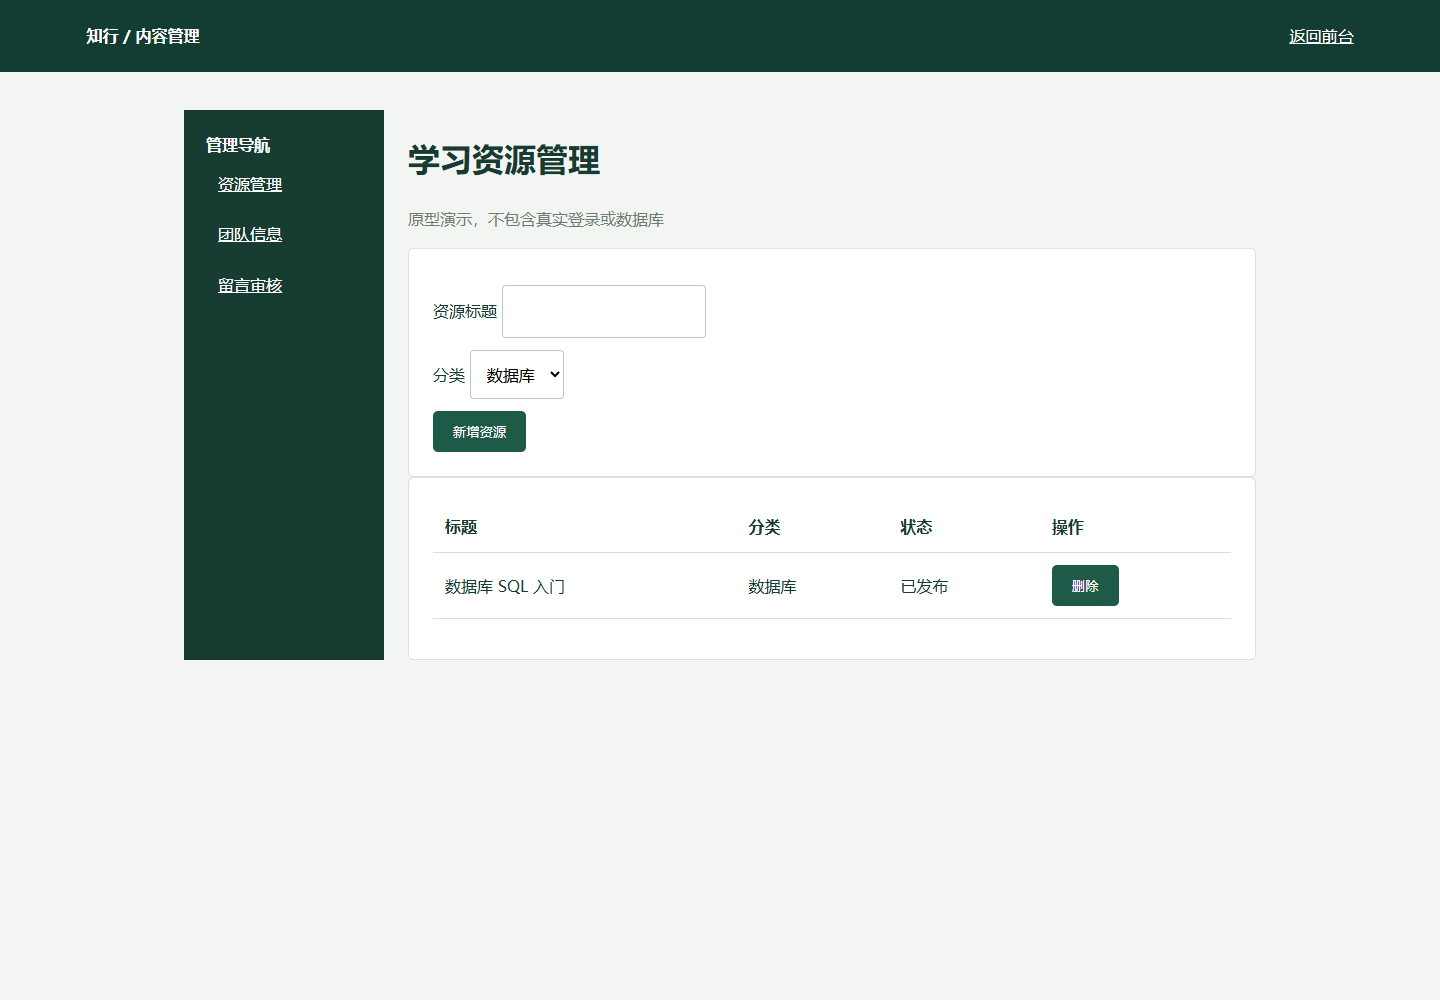
\includegraphics[width=\linewidth,height=.29\textheight,keepaspectratio]{figures/figure-02.png}
\caption{后台资源管理的表单与初始列表}
\end{figure}


\begin{figure}[H]\centering
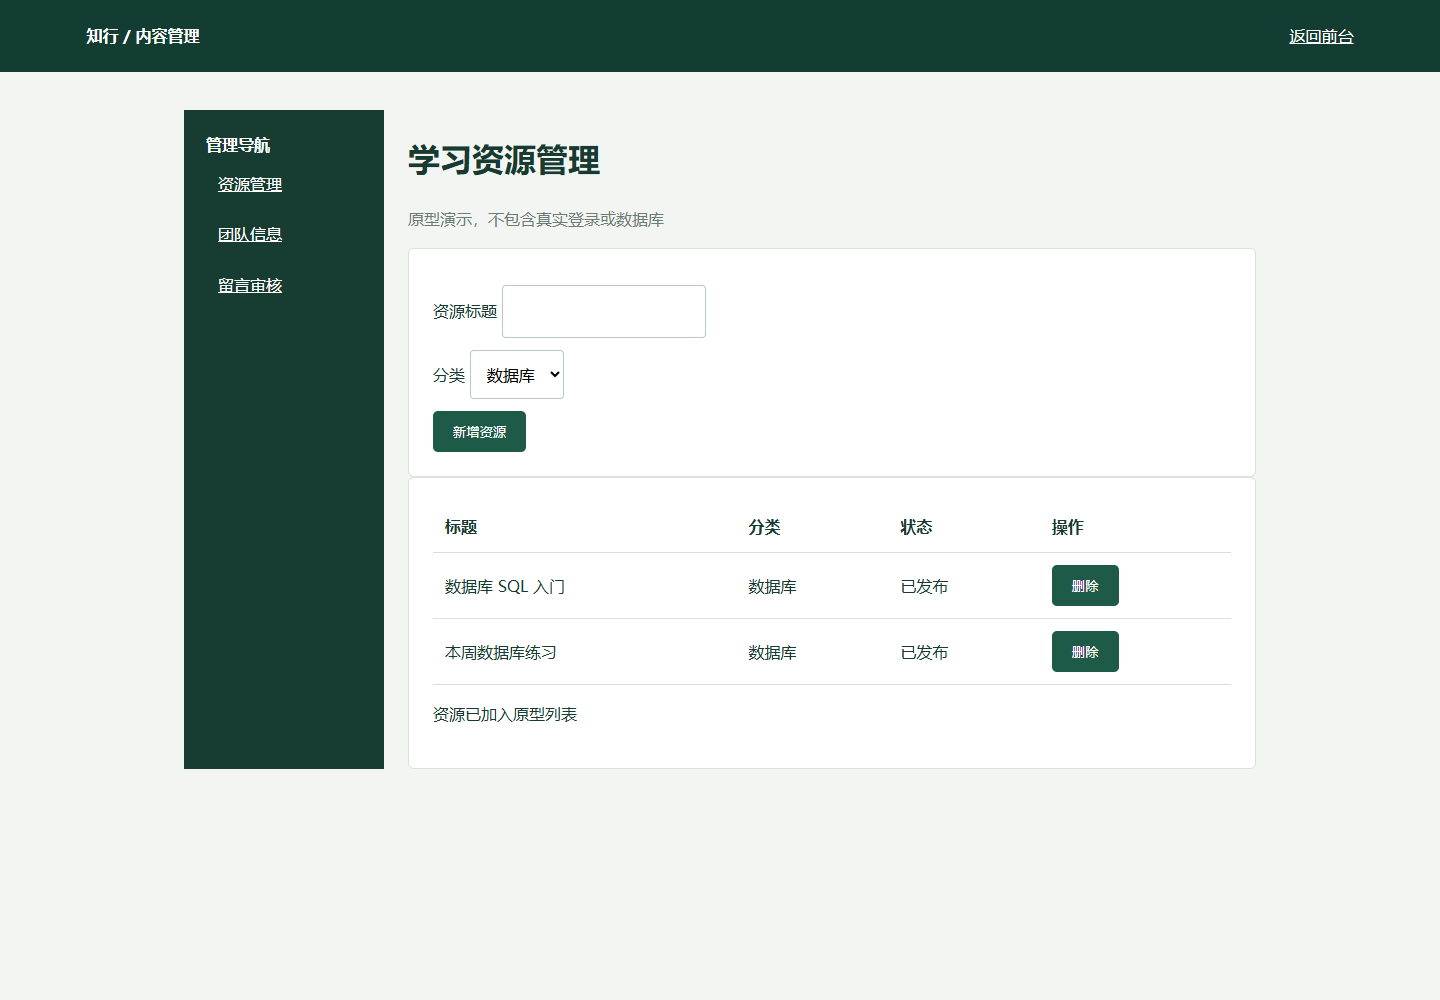
\includegraphics[width=\linewidth,height=.29\textheight,keepaspectratio]{figures/figure-03.png}
\caption{填写表单并提交后的资源列表}
\end{figure}


提交表单后，新增记录显示在列表中，页面同时给出状态反馈。每一行的删除按钮对应当前记录，使操作对象明确。表单与列表上下相邻，可以在完成新增后直接查看结果，也能从列表中选择需要移除的记录。

资源管理原型通过当前页面状态组织这些交互。数据变化只作用于本次打开的页面，刷新后恢复初始记录。这样的呈现方式用于说明管理流程与反馈位置，前台与后台的视觉结构也保持一致。

\section{前后台模板选择}
\subsection{前台模板选择 Agency}
前台选择 Start Bootstrap 的 Agency 单页模板。它以首屏介绍、内容展示、团队和联系区域组织页面，与校园学习团队网站的介绍、资源、成员和留言四类内容相对应。单页结构能够让访客沿页面向下浏览，同时通过导航直接进入所需区域。

模板中的 Services 栏目可对应学习方向，Portfolio 可对应课程资源与项目成果，Team 可对应成员介绍，Contact 可对应留言交流。栏目之间的层次适合先介绍团队，再展示内容，最后提供联系入口的阅读顺序。

\begin{figure}[H]\centering
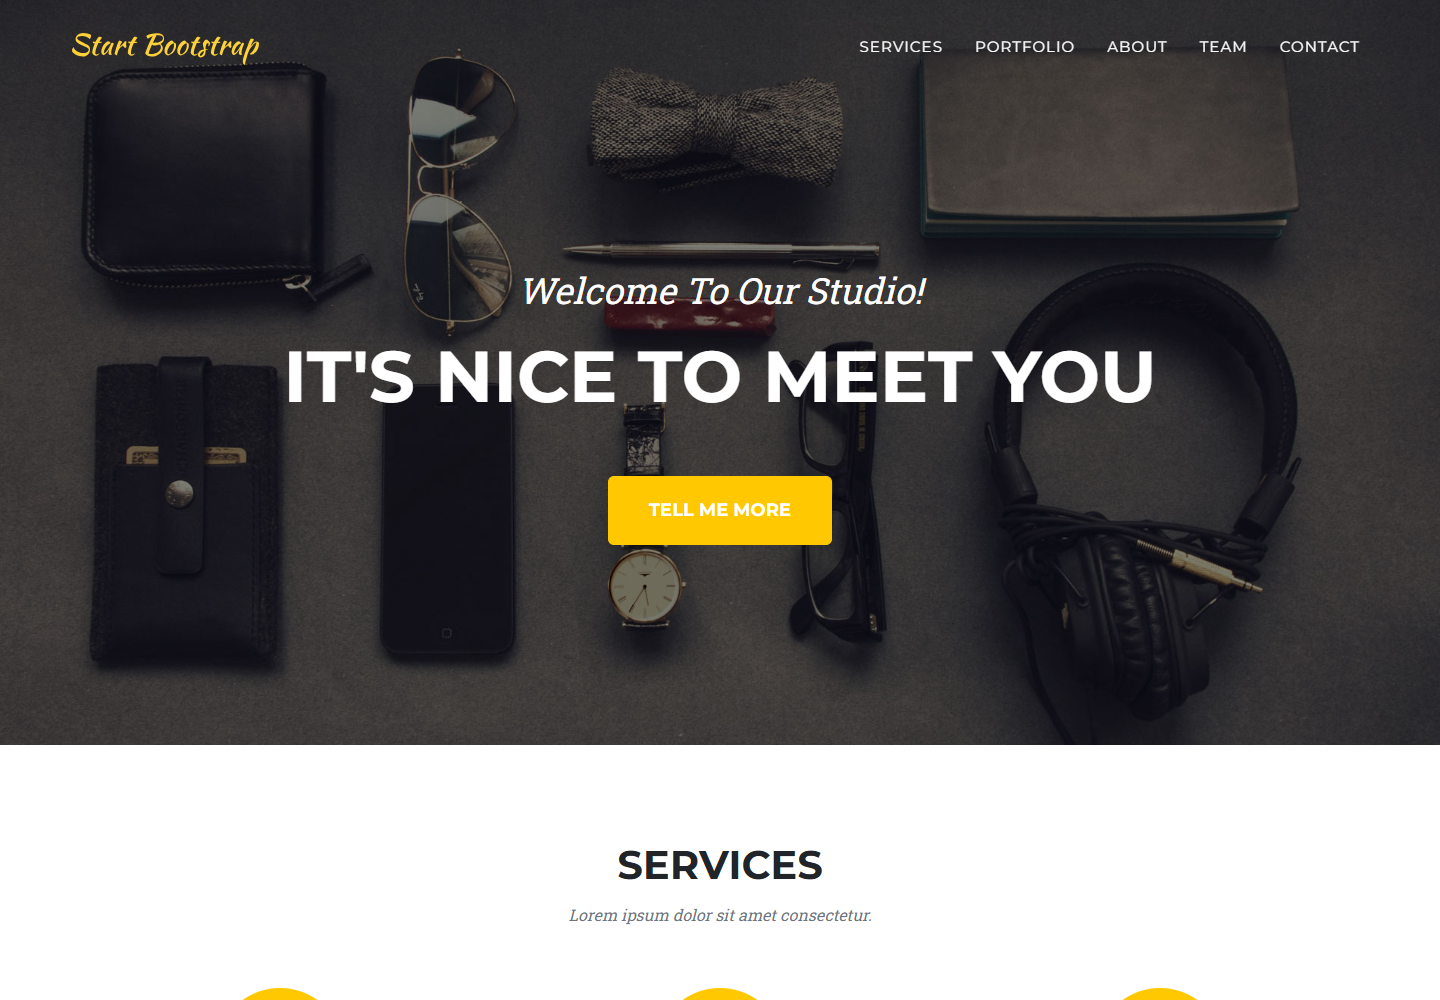
\includegraphics[width=\linewidth,height=.34\textheight,keepaspectratio]{figures/figure-04.png}
\caption{Agency前台模板的首屏与栏目展示}
\end{figure}


模板的首屏具有明确的标题与主要按钮，能够承载团队名称、学习主题和资源浏览入口。资源展示区域可沿用图文卡片，成员区域保留姓名与简介，联系区域放置留言表单。将这些内容对应到原型后，可以保留模板的主要结构，再根据实际栏目调整文字和展示顺序。

\subsection{后台模板选择 Tabler}
后台选择 Tabler 管理模板。后台页面的主要任务是查看记录、填写信息和执行操作，Tabler 提供的导航、表格、表单与状态标签适合这种内容组织方式。其工作区能同时呈现资源概况和详细列表，便于维护者从整体数量转向具体记录。

本地适配页将学习资源、团队成员和示例留言放在概况区域，再以资源列表展示标题、分类和发布状态。概况用于快速了解内容规模，表格用于逐条读取信息。状态标签与正文区分显示，使记录状态能够在浏览列表时直接识别。

\begin{figure}[H]\centering
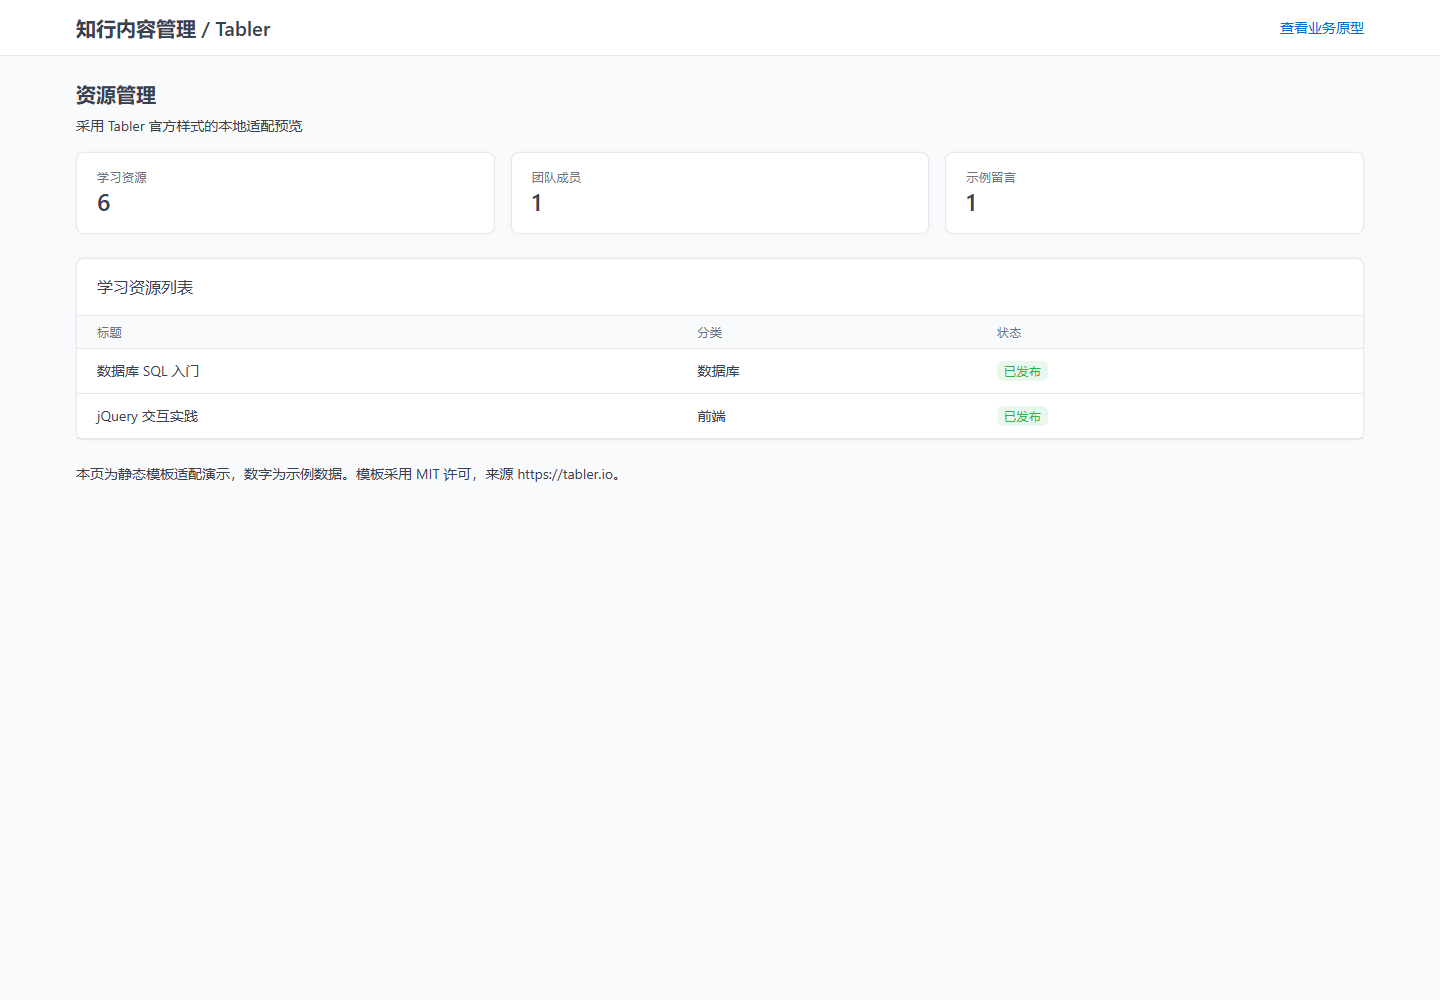
\includegraphics[width=\linewidth,height=.34\textheight,keepaspectratio]{figures/figure-05.png}
\caption{Tabler后台模板的概况区域与资源列表}
\end{figure}


资源管理页面可以沿用这一结构，将原型中的新增表单与列表组合进工作区。表单用于录入标题和分类，列表用于展示和定位记录，操作按钮则与对应行放在一起。Agency承担前台展示，Tabler承担后台管理，两者分别服务于内容浏览和内容维护的任务。

\end{document}
